\documentclass[]{beamer}

\usepackage[T1]{fontenc}
\usepackage[utf8]{inputenc}
\usepackage{ctex}  % 支持中文
\usepackage{graphicx} % 插入图片的包

\usetheme{Boadilla}  % 主题
\usecolortheme{default}  % 主题的颜色

\title{Introduction of A Simplified Crypto Bank}  % 标题
\author[Jingwei Feng, Bowen Li, Zhicheng Gao]{\begin{tabular}{c} 冯镜维 \\ 李博文 \\ 高志成 \end{tabular}}
\date{\today}  % 时间

\begin{document}  % 正文开始

    \begin{frame}  % 相当于ppt里的一页
        \titlepage  % 标题页
    \end{frame}

    \begin{frame}
        \frametitle{Menu}  % 当前页的标题  
        \tableofcontents  % 制作目录,需要\section{}配合
    \end{frame}
    
    \section{总体架构}  % 用来做目录
    \begin{frame}  
        \frametitle{问题分解}  
        \textbf{银行转账}
        \begin{itemize}  
            \item 身份认证
            \begin{itemize}
                \item 注册: 邮箱号,用户名,登录密码,支付密码
                \item 登录: 用户通过输入邮箱和密码进行登录
                \item 用户信息修改(忘记密码)
            \end{itemize}
            \item 银行卡管理
            \begin{itemize}
                \item 开通新银行卡
                \item 多张银行卡,金额独立
            \end{itemize}
            \item 交易
            \begin{itemize}
                \item 存取款(模拟)
                \item 转账
            \end{itemize}
        \end{itemize}
    \end{frame}

    \section{交易}
    \begin{frame}{交易}
        \textbf{方式}
        \begin{enumerate}
            \item Alice与Bob直接通过网上银行进行转账
            \item Bob开了一家牛肉烧麦店,挂在交易平台上,Alice下订单购买
        \end{enumerate}
        \textbf{简单商城} \\[2ex]

        虚拟银行为虚拟商城提供必要的支付接口,虚拟商城用于模拟用户在实际生活中交易的过程。\\[2ex]

        例如 Alice在Bob的网店上订购了一斤烧麦\\[2ex]

        \begin{itemize}
            \item 商城:订单确实存在,而且交易双方的身份不能变
            \item 银行:可信资金平台,Alice确实有足够多的钱,这笔钱确实转给了Bob
        \end{itemize}
    \end{frame}

    \begin{frame}{模块总结}
        \begin{enumerate}
            \item 利用银行来实现转账、存取款
            \item 利用网络商城模块和银行模块的协作来实现交易
            \item 银行和网络商城都需要一套安全的交互协议来保证可信
        \end{enumerate}
    \end{frame}

    \begin{frame}{顶层结构图}
        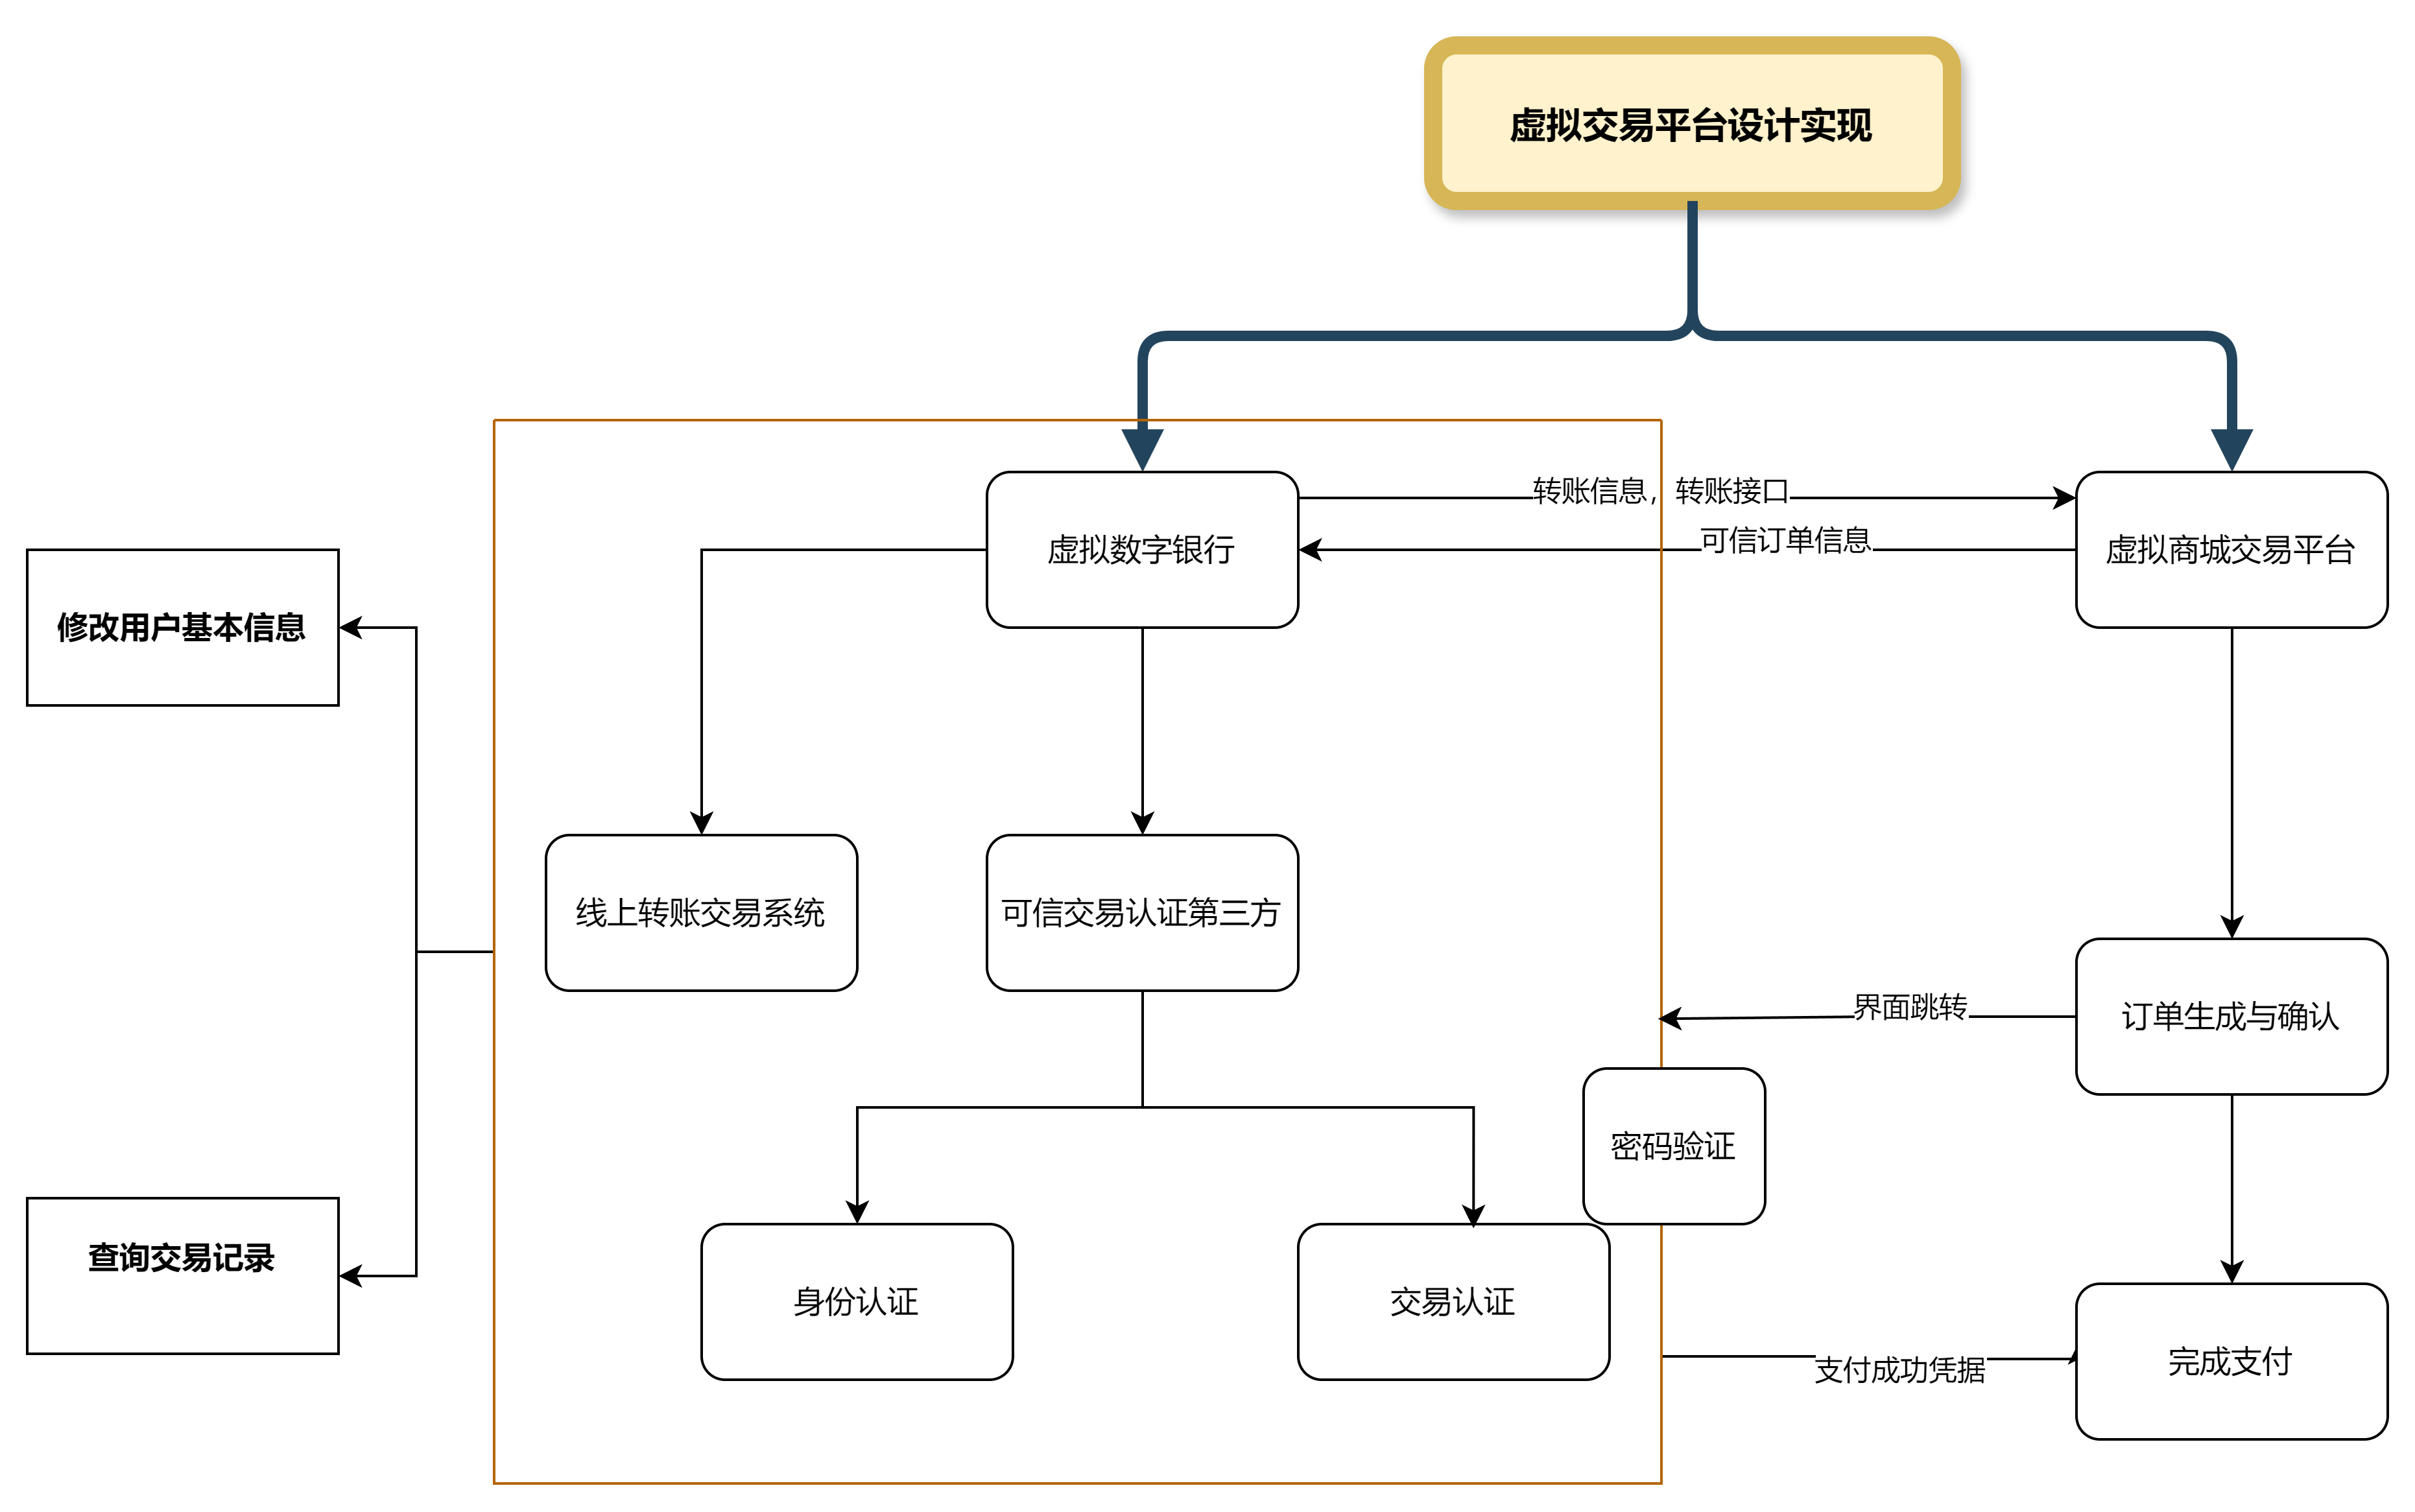
\includegraphics[width=1\textwidth]{module.png}
    \end{frame}
    
    \section{需求分析}  
    \begin{frame}  
        \frametitle{安全需求} 
        \textbf{从攻击者的角度看,哪些地方可以狠狠地攻击}
        \begin{itemize}
            \item 用户信息认证 <- \textbf{unsign, cookie injection,弱口令爆破}
            \item 交易过程 <- \textbf{信息窃听, MIM, 篡改,重放}
            \item 数据处理
            \begin{itemize}
                \item 数据查询过程 <- \textbf{SQL注入}
                \item 数据渲染 <- \textbf{SSRF导致的RCE}
            \end{itemize}
            此外,整个过程还涉及DDOS等一些暴力下三滥手段
        \end{itemize}
    \end{frame}
    
    \begin{frame}{安全需求}
        \textbf{根据刚才列举的简单部分攻击,分析安全需求}
        \begin{enumerate}
            \item 账户安全: 采用\textbf{jwt}严格认证,规范过期时间,对session添加\textbf{唯一id}
            \item 交易过程: 对于商城交易,采用SET协议,对于银行转账,采用AES对交易信息加密,并SHA256生成摘要进行验证,\textbf{确保CCA安全}
            \item 通信安全:使用TLS1.2防范窃听攻击和中间人攻击
            \item 数据处理:采用前后端分离开发,在后端对前端发来的参数请求执行严格的白名单过滤策略
            \item 用户信息安全:规范并强制用户提高密码复杂度以防范简单的弱口令爆破
            \item 针对拒绝服务攻击:严格控制请求次数,构筑基本的防火墙
        \end{enumerate}
    \end{frame}
    
    \section{模块设计}
    \begin{frame}{用户信息认证模块}
        \begin{columns}
            \begin{column}{0.5\textwidth}
                \textbf{用户操作}
                \begin{itemize}
                    \item 注册:实名身份信息认证,登录密码,支付密码,输入唯一用户名以及邮箱,提供唯一用户ID
                    \item 登录:用户通过唯一用户名登录,密码正确即可进入系统
                    \item 忘记密码:通过邮箱重置账号密码
                \end{itemize}
            \end{column}
            \begin{column}{0.5\textwidth}
                \textbf{服务器认证过程}
                \begin{enumerate}
                    \item 对用户信息利用\textbf{jwt}进行封装
                    \item 对支付密码和登录密码用\textbf{SHA256}哈希
                    \item 前端设置好\textbf{cookie}并规范\textbf{ID}和\textbf{过期时间}
                \end{enumerate}
            \end{column}
        \end{columns}
    \end{frame}

    \begin{frame}{认证模块信息交互流程图}   
        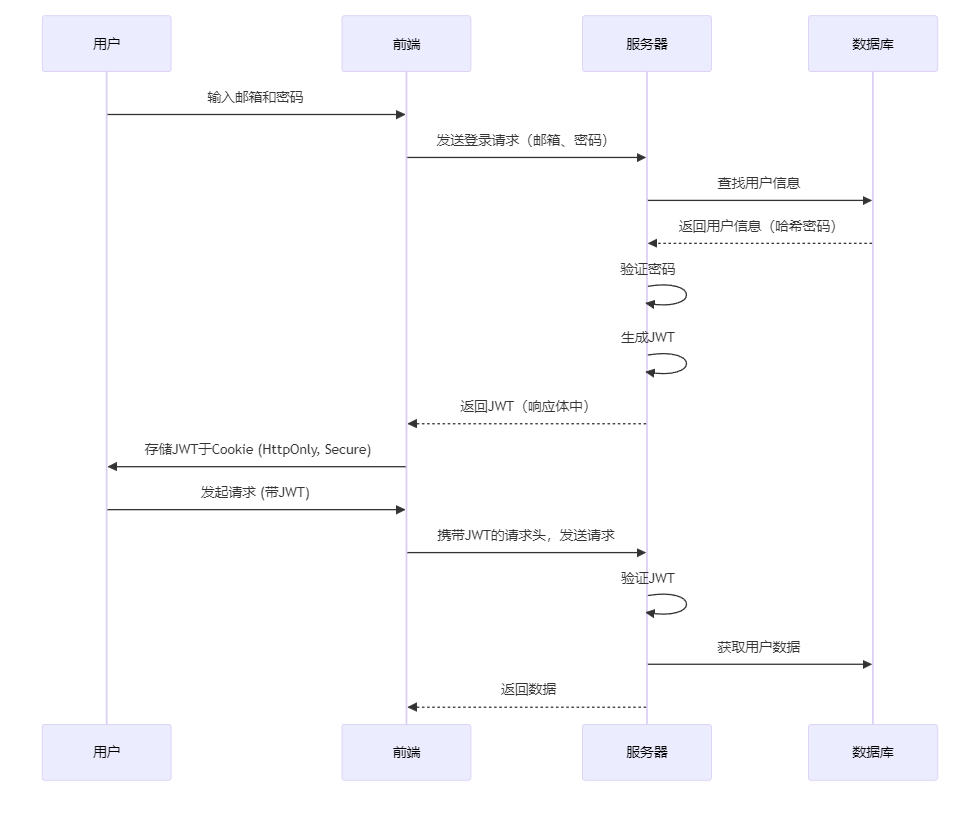
\includegraphics[width = 0.8\textwidth]{newsqe.png}
    \end{frame}

    \begin{frame}{认证模块的额外要求}
        \begin{itemize}
            \item 要有admin账户,对一切用户进行管理
            \item 要求用户有实名认证环节,调用其他可信接口(例如国家信息认证),在本项目中模拟为通过管理员审核
            \item 用户在实名认证前不能进行任何交易操作
        \end{itemize}
    \end{frame}
    
    \begin{frame}{网上交易模块}
                \textbf{银行转账协议的安全设置}
                \begin{itemize}
                    \item \textbf{通信安全}:所有通信都通过\textbf{TLS协议}进行,确保数据在传输过程中的机密性、完整性和真实性,防止中间人攻击
                    \item \textbf{交易加密}:每一笔交易都使用\textbf{AES加密},确保交易数据在存储和传输过程中的安全性
                    \item \textbf{消息摘要}:对交易数据进行\textbf{SHA-256摘要}处理,确保数据在传输和存储过程中未被篡改,防止重放攻击和选择密文攻击(CCA)
                \end{itemize}
    \end{frame}

    \begin{frame}{网上交易的安全流程}
        \begin{enumerate}
            \item 用户通过TLS加密通道连接服务器,发起转账请求
            \item 服务器生成会话密钥,用于本次交易的\textbf{AES加密}
            \item 用户输入交易金额和收款方信息,服务器对数据进行\textbf{AES加密},并生成\textbf{SHA-256摘要}
            \item 将加密后的交易数据和摘要通过\textbf{TLS安全通道}发送给银行
            \item 银行解密交易数据,验证摘要,确保数据的完整性和真实性,然后执行转账操作
            \item 转账完成后,银行生成确认信息,并通过\textbf{TLS安全通道}反馈给用户,确认交易已成功处理
        \end{enumerate}
    \end{frame}
    
    \begin{frame}{交易过程流程图}
        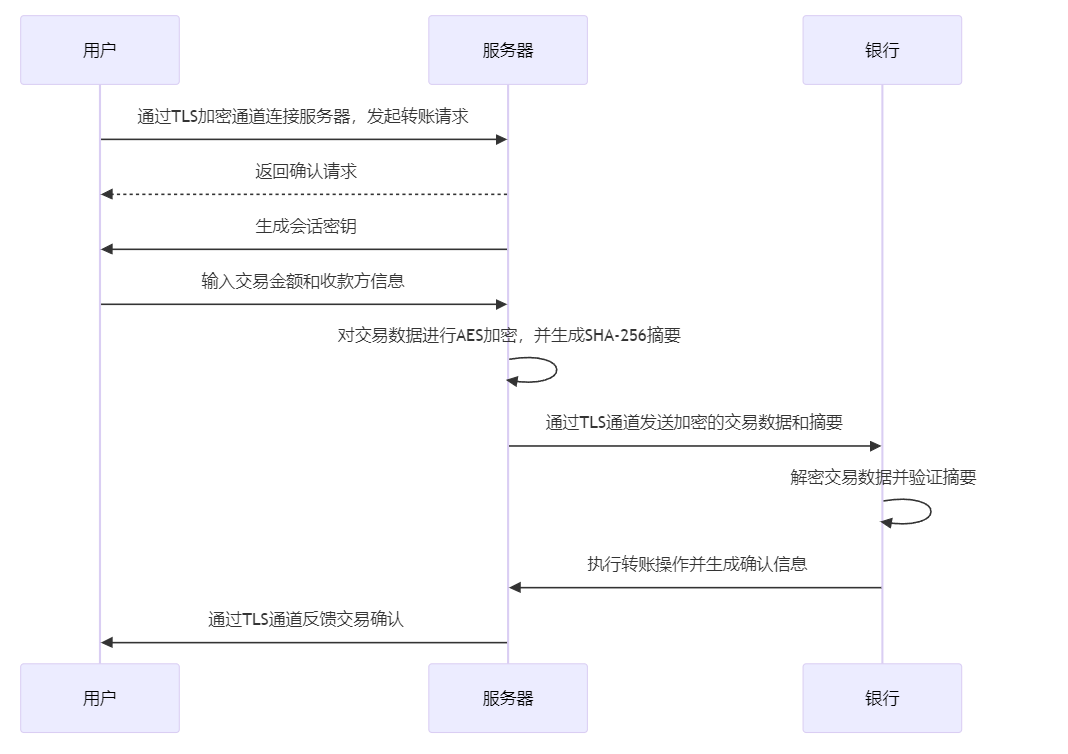
\includegraphics[width=1.0\textwidth]{bank.png}
    \end{frame}
    

    \begin{frame}{存取款操作流程}
        \begin{enumerate}
            \item \textbf{身份验证}:用户通过用户名和密码登录系统。
            \item \textbf{银行卡选择}:用户选择要进行存取款操作的银行卡。
            \item \textbf{银行卡验证}:服务器验证银行卡的真实性。
            \item \textbf{余额检查}(仅取款):系统检查所选银行卡的余额是否足够。
            \item \textbf{存取款操作}:用户输入存款或取款金额,服务器处理操作并反馈交易确认。
        \end{enumerate}
    \end{frame}

    \begin{frame}{存取款信息安全保障}
        \begin{itemize}
            \item \textbf{通信安全}:使用TLS协议确保数据传输安全。
            \item \textbf{数据加密}:对敏感信息进行AES加密处理。
            \item \textbf{数据完整性}:使用SHA-256摘要验证数据完整性。
            \item \textbf{身份验证}:使用JWT严格验证用户身份。
            \item \textbf{会话安全}:为每次交易生成唯一的会话密钥。
        \end{itemize}
    \end{frame}
    
    
    

    \begin{frame}{额外约束}
        \begin{itemize}
            \item 转账双方都需要有至少一张银行卡。
            \item 双方必须在实名认证后才可以申请绑定银行卡,因此在这之后才能转账。
            \item 转账方的银行卡余额必须充足。提款时用户对应的银行卡余额也必须充足。
        \end{itemize}
    \end{frame}

    \begin{frame}{虚拟线上商城}
        \textbf{用户认证} \\
        线上商城只是为了模拟交易过程,因此为了简化用户部分,我们假定这个商城是银行系统的派生产品,因此共用一套用户系统。
    
        \vspace{1em} % 插入一个空行
        
        \textbf{同样,用户只有在实名认证之后,才有权利开张店铺并使用银行系统的各种功能和接口。}
    \end{frame}
    
    \begin{frame}{确保订单安全}

        \setbeamercolor{block title}{bg=purple,fg=white}
        \setbeamercolor{block body}{bg=purple!10,fg=black}
        
        \begin{block}{}
            在订单交易过程中,银行在实质上是一个可信的第三方,用来证明付款人A的银行卡余额充足,且收款人B的银行卡确实存在,并能可信地通知交易平台转账成功,从而结束交易。
        \end{block}
    
        \vspace{1em} % 插入一个空行
    
        在这个过程中,银行模块\textbf{不能查看商家和客户之间的订单信息,只能查看转账信息}。同时要有\textbf{验证订单信息真实性的能力}。
    
    \end{frame}
    
    
    

    \begin{frame}{双签名与SET Protocol}
        
    \end{frame}


\end{document}
